\documentclass[12pt]{article}
\usepackage[a4paper,
	left=1in,
	right=1in,
	top=1in,
	bottom=1in]{geometry}
\usepackage{tikz}
\usetikzlibrary{positioning,arrows}
\usetikzlibrary{decorations.pathmorphing}
\usetikzlibrary{decorations.markings}
\usepackage{gensymb}
\usepackage{amsmath}
\usepackage{cancel}
\usepackage{xcolor}
\usepackage{amssymb}
\usepackage{graphicx}
\usepackage{systeme}
\usepackage{hyperref}
\usepackage{pgfplotstable,filecontents}
\pgfplotsset{compat=1.9}
\usepackage[scaled=0.9]{DejaVuSansMono}
\usepackage{listings}
\usepackage{subcaption}
\usepackage{setspace}
\usepackage{relsize}
\usepackage{bigints}
\usepackage{lscape}
\usepackage{caption}
\usepackage{indentfirst}
\usepackage{amsmath}
\usepackage{sectsty}
\usepackage{textcomp}
\usepackage{gensymb}
\usepackage{mathtools, cuted}
\usepackage{subcaption}
\usepackage{csquotes}
\usepackage{setspace}

\renewcommand\arraystretch{1.5}
\renewcommand{\thefootnote}{\fnsymbol{footnote}}
\sectionfont{\fontsize{12}{15}\selectfont}
\subsectionfont{\fontsize{12}{15}\selectfont}
\subsubsectionfont{\fontsize{12}{15}\selectfont}


\definecolor{codegreen}{rgb}{0,0.6,0}
\definecolor{codegray}{rgb}{0.5,0.5,0.5}
\definecolor{codepurple}{rgb}{0.58,0,0.82}
\definecolor{backcolour}{rgb}{0.95,0.95,0.92}

\renewcommand{\rmdefault}{ptm}

\lstdefinestyle{mystyle}{
	backgroundcolor=\color{backcolour},   
	commentstyle=\color{codegreen},
	keywordstyle=\color{magenta},
	numberstyle=\tiny\color{codegray},
	stringstyle=\color{codepurple},
	basicstyle=\ttfamily\scriptsize,
	breakatwhitespace=false,         
	breaklines=true,                 
	captionpos=b,                    
	keepspaces=true,                 
	numbers=left,                    
	numbersep=5pt,                  
	showspaces=false,                
	showstringspaces=false,
	showtabs=false,                  
	tabsize=4
}
\lstset{style=mystyle}

\doublespacing
\setlength\parindent{24pt}

\tikzset{
	particle/.style={thick,draw=black, postaction={decorate},
		decoration={markings,mark=at position .5 with {\arrow[black]{triangle 45}}}},
	gluon/.style={decorate, draw=black,
		decoration={coil,aspect=0}}
}


\begin{document}

\section*{CHAPTER II\centering\\REVIEW OF RELATED LITERATURE}

This section presents the review of related literature and studies regarding the mechanisms and theoretical principle of RFID, electromagnetism, algorithms and the programming languages, and the derivation of the equations presented in the later section.

According to Standard Model of Quantum Physics (Kibble, 2015) the electromagnetic waves carried by quanta of photons, $\gamma$, are product of interactions by electrons ($e^{-}$) as shown by Feynman diagram below:
	
	\begin{figure}[h]
		\begin{center}
			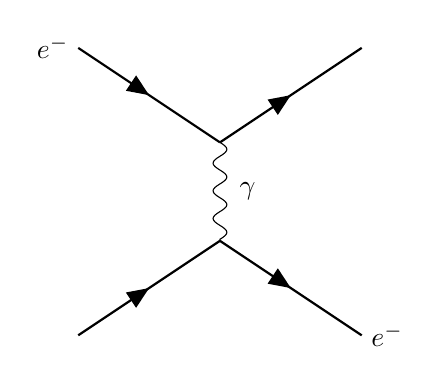
\begin{tikzpicture}[node distance=1.2cm and 1.8cm] \centering
				\coordinate[label=left:$e^{-}$] (e1);
				\coordinate[below right=of e1] (aux1);
				\coordinate[above right=of aux1] (e2);
				\coordinate[below=1.25cm of aux1] (aux2);
				\coordinate[below left=of aux2] (e3);
				\coordinate[below right=of aux2,label=right:$e^{-}$] (e4);
				
				\draw[particle] (e1) -- (aux1);
				\draw[particle] (aux1) -- (e2);
				\draw[particle] (e3) -- (aux2);
				\draw[particle] (aux2) -- (e4);
				\draw[gluon] (aux1) -- node[label=right:$\gamma$] {} (aux2);
			\end{tikzpicture}
		\end{center}
		\caption{Electron-electron interaction as shown by Feynman's diagram.}	
		\label{fig:1}
	\end{figure}
	
Where as the wave function, $\phi(\{\boldsymbol{r_i \sigma_i}\})$, and its energy, $E^{e}_{v}$ are determined by the equation:

	\begin{equation}
		H^{e} = \mathlarger{\sum_{k=1}^{N}} - \frac{\hbar}{2m} \nabla^{2}_{r_{k}} + \mathlarger{\sum_{k=1}^{N}} v(\boldsymbol{r_{k}}) + \frac{1}{2} \frac{1}{4\pi \epsilon_{0}} \mathlarger{\sum_{\substack{k, k'\\k=1}}^{N}} + \frac{e^{2}}{|\boldsymbol{r_{k}} - \boldsymbol{r_{k'}}|}
	\end{equation}

Since light is a dual nature, hence the term “wave-particle duality of light” (Giancoli, 2016; Kibble, 2015), which can be shown with Einstein’s equation, as energy and mass is interchangeable entity, it can used as a method for efficient information transfer.

Considering an object with mass, $m_0$, and assuming that it moves under the influence of force, $F$. According to the Work-Energy theorem, the change in energy, $E$, is the work done by force, $F$ :

\begin{equation}
	E = \bigintss_{0}^{x} F\;dx
\end{equation}

Since $F = ma$ : 

\begin{align*}
	F &= \frac{d}{dt_1} (m_1 v_1) = \frac{d}{dt_1} \Biggr ( \frac{m_0 v_1}{\sqrt{1 - \frac{v^2_1}{c^2_1}}} \Biggr ) \longrightarrow \frac{m_0 a_1}{\Big (1 - \frac{v_1^2}{c_1^2}  \Big )^{3/2}}
\end{align*}

As if the mass change then force, $F$, is changed in momentum $F = \frac{d}{dt}(mv)$. Then it follows that:

\begin{align*}
	E = \bigintss_{0}^{x} F\;dx &= \bigintss_{0}^{x} \frac{m_0 a_1}{\bigg ( 1 - \frac{v_1^2}{c_1^2} \bigg )^{3/2}} \;dx \\
	&\Longrightarrow m_0 \bigintss_{0}^{x} \frac{a_1}{\bigg ( 1 - \frac{v_1^2}{c_1^2} \bigg )^{3/2}}\;dx
\end{align*}

Since :

\begin{equation*}
	a_1 = \frac{dv_1}{dt_1} = \frac{dv_1}{dx} \frac{dx}{dt_1} = v_1 \frac{dv_1}{dx}
\end{equation*}

Through substitution $E$ can be rewritten as:

\begin{align}
	E &= m_0 \bigintss_{0}^{x} \frac{v_1}{\bigg ( 1 - \frac{v_1^2}{c^2} \bigg )^{3/2}} \frac{dv_1}{dx}\;dx \nonumber \\
	E &= m_0 \bigintss_{0}^{v_1} \frac{v_1}{\bigg ( 1 - \frac{v_1^2}{c^2} \bigg )^{3/2}}\;dv_1 \label{d:1}
\end{align}

And finally:

\begin{equation}
	E = c^2 (m_1 - m_0) \longrightarrow \Delta m c^2
\end{equation}

The RFID then utilizes the electromagnetic particles and wave described previously, whereas it carries information based on the wavelength, $\lambda = \frac{c}{f}$, and velocity of the particle. While the matter-energy interaction can further be described using different set of equations, that is deemed not necessary in this review.


While the information sent by the RFID receiver, the processing happens in computer, as the information needs to be further processed for utilization, since in the most basic form it is an entropy which is defined as (McDonnell \& Ikeda, 2011):

\begin{equation}
	H(X) = -E_{p(X)} [\boldsymbol{log} p(x)]
\end{equation}

And since information is also a system contained in a universe, it is also assumed to dissipate over time. Zak (2018) mathematically modeled the heat death of universe using the law of thermodynamics that describes the entropy. Madalung (1926) cited by Zak (2018) modeled the hydrodynamics version of the Schrodinger equation through, in which the quantum potential and the classical potential can be seen, last term and $F$:

\begin{align}
	\frac{\partial S}{\partial t} + \nabla \bullet \Big ( \frac{\rho}{m} \nabla S \Big ) = 0 \label{s1} \\
	\frac{\partial S}{\partial t} + (\nabla S)^2 + F - \frac{\hbar^2 \nabla^2 \sqrt{\rho}}{2m \sqrt{\rho}} = 0 \label{s2}
\end{align}

Where $\rho$ and $S$ are the components of wave function, $\Psi = \sqrt{\rho e}^{i\frac{S}{\hbar}}$ and planck constant, $\hbar$ divided by $2\pi$. And by using ansats, Madelung equations can be converted into Schrodinger equation :

\begin{align*}
	\sqrt{\rho} = \Psi exp(-i \frac{S}{\hbar})
\end{align*}

Using Liouville equation:

\begin{equation}
	\frac{\partial \rho}{\partial t} + \nabla \bullet (\rho F) = 0
\end{equation}

Which was used to generalized the concept of probablity, $\rho$, generated by system of ordinary differential equations, $\frac{dv}{dt} = F[v_1 (t), v_2(t), \dots v_n (t), t]$:

\begin{align}
	\frac{dv}{dt} &= F[p(v)] \label{s3} \\
	\frac{\partial \rho}{\partial t} + \nabla \bullet {\rho F[p(v)]} &= 0 \label{s4}
\end{align}

Equation 9 was generated using Liouville equation generated by Equation 10, which is in contrast to  $\frac{\partial \rho}{\partial t} + \nabla \bullet (\rho F) = 0$, nonlinear with respect to the probability density, $\rho$.

Following the derivation made by Zak (2016), the force, $F$ that plays the role of feedback from Liouville equation, to the:

\begin{align}
	F &= c_0 + \frac{1}{2}_1 \rho - \frac{c_2}{\rho} \frac{\partial \rho}{\partial v} + \frac{_3}{\rho} \frac{\partial ^2}{\partial v^2} \label{s5} \\
	& c_0 > 0, c_1 > 0, c_3 > 0 \nonumber
\end{align}

Then through reduction, it transforms into :

\begin{equation}
	\ddot{v} = c_0 + \frac{1}{2}_1 \rho - \frac{c_2}{\rho} \frac{\partial \rho}{\partial v} + \frac{_3}{\rho} \frac{\partial ^2}{\partial v^2} \label{f} \\
\end{equation}

And then the Liouville equation will transform into :

\begin{equation*}
	\frac{\partial \rho}{\partial t} + (c_0 + c_1 \rho)\frac{\partial p}{\partial V} - c_2 \frac{\partial ^2}{\partial V^2} + c_3 \frac{\partial ^3 \rho}{\partial V^3} = 0
\end{equation*}

This equation is known as kdV-Burgers (Korteweg-deVries-Burgers) partial differential equation (PDE) :

\begin{equation*}
	\bigintss_{-\infty}^{\infty} \rho dV = 1 \nonumber
\end{equation*}

And finally the final change in entropy can be show by assuming that the simplest cases of the system that is $c_0 = 0, c_2 = 0, c_3 = 0, c_1 > 0$ :

\begin{align}
	\frac{\partial H}{\partial t} &= - \frac{\partial}{\partial t} \bigintss_{-\infty}^{\infty} \rho ln \rho dV = - \bigintss_{-\infty}^{\infty} \dot{\rho} (ln \rho + 1) dV \nonumber \\
	&= \bigintss_{-\infty}^{\infty} \frac{1}{2} c_1 \frac{\partial}{\partial V} (\rho ^2) (ln \rho + 1)dV \nonumber \\
	&= \frac{1}{2} c_1 \bigg [  \rvert_{-\infty}^{\infty} \rho ^2 (ln \rho + 1) - \int_{-\infty}^{\infty} \rho dV \bigg ] = \frac{1}{2} c_1 < 0 
\end{align}

This difference called \textit{Schr$\dot{o}$dinger paradox} : in a system obeying the second law of thermodynamics, all isolated system, such as this universe, is expected to reach a state of maximum disorder (Zak, 2018).

Thus, to read the information sent by the RFID, computers are necessary, since information is entropy.

Reading the information can be done using programming language, as it is a well established basic fact that kernel interaction is the precedence of programming language or machine language interaction with the input, usually by C and C++ in operating systems, creating a
closed loop of: interface $\longrightarrow$ programming langauge response $\longrightarrow$ kernel $\longrightarrow$ hardware $\longleftarrow$ interface $\longrightarrow$ \dots.

Programming languages can be used efficiently with algorithms, which is defined as a set of instructions for a certain task. One exemplification is its utilization in Machine Learning,
also known as computational learning theory (Letvina et al., 2021).
	
One of the other prominent regression algorithm is logistic algorithm which is used for explanation of relation of independent and dependent variable, as shown below:
	

\begin{align}
	\nabla J(\theta) &= \theta + \mathlarger{\sum^{m}_{i=1}} \frac{exp \bigg( \bigg \langle  -y_i \hat{\phi} (x_i), \theta \bigg \rangle \bigg)}{1 + exp \bigg(\bigg \langle  -y_i \hat{\phi} (x_i), \theta \bigg \rangle \bigg )} (-y_i \hat{\phi} (x_i)) \nonumber \\
	&= \theta + \mathlarger{\sum^{m}_{i=1}} (p(y_i|x_i, \theta) - 1)y_i \hat{\phi}(x_i) \nonumber
\end{align}

then, the Hessain can be computed :

\begin{align}
	\nabla ^2 (\theta) = I - \mathlarger{\sum^{m}_{i=1}}p (y_i|x_i, \theta) (1 - p (y_i|x_i, \theta) \hat{\phi} (x_i) \hat{\phi} (x_i)^\top
\end{align}

Simple linear regression on the other hand, which was the regression model the study used, can be derived as follows. Since the direct regression approach minimizes the sum of squares :

\begin{align*}
	S(\beta_0, \beta_1) = \mathlarger{\sum^{n}_{i+1}} \varepsilon^2_i = \mathlarger{\sum^{n}_{i=1}} (y_i - \beta_0 -\beta_1 x_i)^2 \nonumber 
\end{align*}

Then the partial derivations of $S(\beta_0, \beta_1)$ with respect to $\beta_0$, and with respect to $\beta_1$, can be solved as Equation 2, and 3, respectively : 

\begin{align}
	&\frac{\partial S(\beta_0, \beta_1)}{\partial \beta_0} = -2 \mathlarger{\sum^{n}_{i=1}} (y_t - \beta_0 - \beta_1 x_i) \\ 
	&\frac{\partial S(\beta_0, \beta_1)}{\partial \beta_1} = -2 \mathlarger{\sum^{n}_{i=1}} (y_t - \beta_0 - \beta_1 x_i) x_i 
\end{align}

The solutions of the two equations are called direct regression estimators, or orginary least squares estimators of $\beta_0$ and $\beta_1$. 

\begin{align*}
	\frac{\partial ^2 S(\beta_0, \beta_1)}{\partial \beta_0^2} &= -2 \mathlarger{\sum^{n}_{i=1}} (-1) = 2n \\
	\frac{\partial ^2 S(\beta_0, \beta_1)}{\partial \beta_1^2} &= 2 \mathlarger{\sum^{n}_{i=1}} x^2_i \\ 
	\frac{\partial ^2 S(\beta_0, \beta_1)}{\partial \beta_0^2 \partial \beta_1} &= 2 \mathlarger{\sum^{n}_{i=1}} x_t = 2n\bar{x} 
\end{align*}

The Hessian matrix, is then given as :

\begin{align}
	H^\ast &= \begin{pmatrix}
		\mathlarger{\frac{\partial ^2 S(\beta_0, \beta_1)}{\partial \beta_0^2}} & \mathlarger{\frac{\partial ^2 S(\beta_0, \beta_1)}{\partial \beta_0^2 \partial \beta_1}} \\[1em]
		\mathlarger{\frac{\partial ^2 S(\beta_0, \beta_1)}{\partial \beta_0^2 \partial \beta_1}} & \mathlarger{\frac{\partial ^2 S(\beta_0, \beta_1)}{\partial \beta_1^2}}
	\end{pmatrix} \\
	&= 2 \begin{pmatrix}
		n & n \bar{x} \\ 
		n \bar{x} & \mathlarger{\sum^{n}_{i=1}} x^2_i         
	\end{pmatrix} \\
	&= 2 \begin{pmatrix}
		\ell ' \\
		x'
	\end{pmatrix} (\ell, x)
\end{align}

The matrix $H^\ast$ is a positive definite if its determinant and the element in the first row and column of $H^\ast$ are positive. The determinant of $H^\ast$ is given by:

\begin{align}
	|H^\ast| &= 4 \bigg ( n  \mathlarger{\sum^{n}_{i=1}} x_i^2 - n^2 \bar{x} ^2 \bigg ) \\
	&= 4n \mathlarger{\sum^{n}_{i=1}} (x_i - \bar{x})^2 \\ 
	&\leq 0
\end{align}

The the equation or the fitted line or the fitted linear regression model is :

\begin{equation}
	y = b_0 + b_i x
\end{equation}

where $\beta_0$ or $b_0$ is the processed value of dependent variable, and $\theta_1, \theta_2, \dots, \theta_n$ are the parameters. Based on this, the regression model were defined, $\mathbf{y_i} = m\mathbf{x_i} + b$, where the algorithm will learn the hypothesis using the existing given dataset to predict $\mathbf{y_i}$ using $\mathbf{x_i}$ and the parameters of the hypothesis, $\theta_1, \theta_2, \dots, \theta_n$, that can be presented in matrix form :

\singlespacing
\begin{align}
	\mathbf{x_i} &= \begin{pmatrix}
		x_{11} & x_{32} & . & . & . & . & x_{1n} \\
		x_{21} & x_{32} & . & . & . & . & x_{2n} \\
		x_{31} & x_{32} & . & . & . & . & x_{3n} \\
		. & . & . & . & . & . & . \\
		. & . & . & . & . & . & . \\
		x_{m1} & x_{m2} & . & . & . & . & x_{mn} \\
	\end{pmatrix} & \theta &= \begin{pmatrix}
		\theta_0 \\
		\theta_1 \\
		. \\
		. \\
		\theta_j \\
		. \\ 
		. \\
		\theta_{m} \\ 
		\theta_{n}
	\end{pmatrix}_{n+1,1} & \mathbf{y} &= \begin{pmatrix}
		y_1 \\
		y_2 \\
		. \\
		. \\
		y_j \\
		. \\ 
		. \\
		y_{m}  \\ 
		y_{n}
	\end{pmatrix}_{m,1}  
\end{align}

\newpage
\section*{CHAPTER III\centering}

This chapter presents the complete description of all procedures in the conduct of the study. 

\subsection*{RESEARCH METHODOLOGY\centering}

\subsubsection*{Device Engineering}
\doublespacing

The lock access and attendance system works similarly to each other in regards of input process. The receiver takes the information or the fingerprinting of the RFID card and relay it to the arduino, while the camera and the RFID information is relayed on to the host system, in case of attendance system.

	\begin{figure}[h!]
		\begin{subfigure}{.5\textwidth}
			\centering
			\includegraphics[width=.4\linewidth]{fig_4.png}
			\caption{Mechanism of RFID-based lock access.}
			\label{fig:sub1}
		\end{subfigure}
		\hfill
		\begin{subfigure}{.5\textwidth}
			\centering
			\includegraphics[width=.4\linewidth]{fig_3.png}
			\caption{Mechanism of the RFID-based attendance device.}
			\label{fig:sub1}
		\end{subfigure}
		\caption{Mechanism of arduino based systems. (a.) shows the mechanism of RFID-based lock system, while (b.) shows the mechanism of RFID-based attendance system.}
	\end{figure}

However, it differs in the process of systemically verifying and checking the information received. Figure 1 exhibits the checking proccess of the RFID-based lock access, and Figure 2 exhibits the checking proccess of the RFID-based attendance system. The RFID-based lock access checks the information natively using the code embded in its arduino, written in C++20 with aid of \texttt{Arduino.h} and various modules. 

On contrary to the RFID-based attendance system, whereas it needs a large database of students and teachers information, it is necessary to use a larger system, which is the host computer. The arduino relays it to the host computer, which would be intercepted by \texttt{systemd} service and relay to the shell, and finally to the checking algorithm written in Python.

\subsubsection*{RFID-based lock system algorithm}

As shown from Figure 1a, the RFID-based locking system uses the native C++20 code inserted to the arduino board, as opposed to the RFID-based attendance that relays the RFID card information to the main system.

\begin{figure}[h!]
	\centering
	\includegraphics[scale=0.6]{fig_2.png}
	\caption{RFID-based lock system algorithm.}
\end{figure}

\subsubsection*{RFID-based attendance algorithm}

The main algorithm, as shown in the Figure 3 below, of the system will be written in \texttt{Python -v 3.9.1} and C++20 with \texttt{Arduino.h} with the student database stored offline in JavaScript Object Notation (JSON) file.

\begin{figure}[h!]
	\centering
	\includegraphics[scale=0.6]{fig_1.png}
	\caption{Algorithm of RFID-based Attendance.} \label{fig:4}
\end{figure}

There are various third party modules used to aid the python standard library was for successful execution of the function. \texttt{pandas.DataFrame()} was used for attendance of the students, as well as \texttt{pandas.to\_excel} function for reporting done to teachers through email everyday. The email was sent using \texttt{Python}'s \texttt{smtplib} and \texttt{ssl}, Simple Mail Transfer Protocol, and Secure Sockets Layer, respectively.

\texttt{git} repository was also setup to be able to modify the data through graphical interface, whereas an updated was pulled every $24 hours$ by a defined \texttt{systemd} service using Linus Torvald's \texttt{git}. By iterating over the JSON database of the student ID and teacher's email address to be used for cases of intruders, the checking was performed.

Then an equation was devised to compare two strings. ID comparison system works by comparing the percent difference of two strings using \texttt{SequenceMatcher} function provided by \texttt{difflib} :

\begin{equation}
	\%_{difference} = \frac{|x_{\forall \in \{\theta_1\}} \equiv y_{\forall \in \{ \theta_2\}}|}{\sum \theta\;|\; N_{\theta_{1}} + N_{\theta_{2}}}
\end{equation}

Since the \texttt{difflib.SequenceMatcher()} does not make error, the value of $\%_{difference}$ should always be equal to 1. Otherwise, the system would recognize the input as an intruder or unregistered student, which would send an alert to the respective teacher of the student.

\newpage
\section*{STATISTICAL TREATMENT AND ANALYSES}

To study the cost efficiency of the RFID-based systems, a regression model was established. Where the algorithm will learn the hypothesis, $\mathbf{h}$ using the existing given data set that it can be used to predict $\mathbf{y_i}$ using $\mathbf{x_i}$ and the parameters of the hypothesis, $\theta_1, \theta_2, \dots, \theta_n$, in an equation form of : $h_\theta (\mathbf{x_i}) = \theta_n + \theta_o (\mathbf{x_i})$.

The regression model was based on the previous prices of materials used for the device, and traditional tools needed (e.g. Attendance book, padlock, etc.). The data were preprocessed with goal of increasing its sensitivity to be able to capture the precision and accuracy in the regression model :


\begin{equation}
	\beta_f = \frac{\beta_i}{\mathbf{ln}(\sqrt{\beta_i})} + |(\theta_1 - \theta_2)|
\end{equation}	
	
\end{document}